% Автоматаар үүсгэсэн — эх файл: lab07/README.md
\chapter{Лаб 7 — Хэрэглээний давхарга ба Zero Trust}

\begingroup\scriptsize\begin{longtable}[]{@{}
  >{\raggedright\arraybackslash}p{(\columnwidth - 2\tabcolsep) * \real{0.5000}}
  >{\raggedright\arraybackslash}p{(\columnwidth - 2\tabcolsep) * \real{0.5000}}@{}}
\toprule
\endhead
\bottomrule
\endlastfoot
\textbf{7 хоног} & XIV \\
\textbf{Хугацаа} & 4 цаг \\
\textbf{Суралцахуйн үр дүн} & ҮД3 (үнэлэх), ҮД4 (аюулгүй зохиох), ҮД6 \\
\textbf{Үнэлгээ} & Бичгийн тайлан, 10 оноо \\
\textbf{Гол хэмжилт} & REST vs GraphQL, аюулгүй байдлын 9 шалгалт (засварын өмнө/дараа) \\
\end{longtable}\endgroup

\hypertarget{ux437ux43eux440ux438ux43bux433ux43e}{%
\section{1. Зорилго}\label{ux437ux43eux440ux438ux43bux433ux43e}}

Платформын дээр \textbf{хэрэглэгчийн давхаргыг} барьж, дараа нь түүнийг \textbf{эвдэхийг оролдоно}.

\begin{enumerate}
\def\labelenumi{\arabic{enumi}.}
\tightlist
\item
  \textbf{Барих} --- REST ба GraphQL-ийн ялгааг зохион бүтээх замаар ойлгох, Dex-ээр OIDC нэвтрэлт, RBAC үүрэг, бодит хугацааны шинэчлэл
\item
  \textbf{Эвдэх} --- \texttt{security\_\allowbreak{}tests.\allowbreak{}py}-г ажиллуулж эмзэг байдлыг олох, гараар батлах, \textbf{засах}, дахин ажиллуулж засварыг нотлох
\end{enumerate}

\begin{quote}
\textbf{Чухал:} \texttt{lab07/\allowbreak{}graphql-api/\allowbreak{}main.\allowbreak{}py} дотор \textbf{ЯГ ХОЁР санаатай эмзэг байдал} бий: \textbf{(А)} \texttt{decode\_token} токены гарын үсэг ба хугацааг шалгадаггүй (\texttt{jwt.\allowbreak{}get\_\allowbreak{}unverified\_\allowbreak{}claims}); \textbf{(Б)} introspection нээлттэй, асуулгын нийлмэл байдлын хязгаар байхгүй. Тэдгээрийг олж засах нь энэ лабораторийн гол ажил. \texttt{security\_\allowbreak{}tests.\allowbreak{}py} (А)-г \textbf{2 ноцтой} (critical/high) УНАСАН мөрөөр, (Б)-г 2 АНХААР мөрөөр харуулна. Лабораторийн эцэст "Санаатай эмзэг байдал илрээгүй" гэж хэвлэж, (Б)-ийн хоёр мөр ТЭНЦСЭН болсон байх ёстой.
\end{quote}

\textbf{{[}ЗК{]} Энэ лаборатори бүхэлдээ үүлний давхаргад.} GraphQL API (:8000), Dex (:5556), бүртгэл (:8090), InfluxDB (:8181) --- бүгд зөөврийн компьютер дээр. {[}Pi{]} Pi 3B нь зөвхөн ирмэгийн үүргээ гүйцэтгэнэ (mosquitto + агент). Pi дээр энэ лабораторид ажиллуулах комманд \textbf{байхгүй} --- гэхдээ агент нь ажиллаж байх ёстой, эс бөгөөс InfluxDB-д унших өгөгдөл байхгүй.

\hypertarget{ux443ux440ux44cux434ux447ux438ux43bux441ux430ux43d-ux43dux4e9ux445ux446ux4e9ux43b}{%
\section{2. Урьдчилсан нөхцөл}\label{ux443ux440ux44cux434ux447ux438ux43bux441ux430ux43d-ux43dux4e9ux445ux446ux4e9ux43b}}

\begin{itemize}
\tightlist
\item
  Лаб 1--6 дууссан, \texttt{lab06-done} tag тавигдсан
\item
  Бие даалт XIV: OAuth2 / OIDC-ийн authorization code урсгалыг уншсан
\end{itemize}

\begin{Shaded}
\begin{Highlighting}[]
\CommentTok{\# [ЗК] үүлний давхаргыг app профайлтай асаана}
\BuiltInTok{cd}\NormalTok{ \textasciitilde{}/cnc302/stack }\KeywordTok{\&\&} \ExtensionTok{docker}\NormalTok{ compose }\AttributeTok{{-}{-}profile}\NormalTok{ core }\AttributeTok{{-}{-}profile}\NormalTok{ pipeline }\AttributeTok{{-}{-}profile}\NormalTok{ app up }\AttributeTok{{-}d} \AttributeTok{{-}{-}build}
\FunctionTok{make}\NormalTok{ health                                          }\CommentTok{\# бүх мөр 200}
\ExtensionTok{curl} \AttributeTok{{-}s}\NormalTok{ localhost:8000/health }\KeywordTok{|} \ExtensionTok{jq}                   \CommentTok{\# \{"status":"ok","checks":\{...200\}\}}
\ExtensionTok{curl} \AttributeTok{{-}s}\NormalTok{ localhost:5556/dex/.well{-}known/openid{-}configuration }\KeywordTok{|} \ExtensionTok{jq}\NormalTok{ .issuer}

\CommentTok{\# [Pi] Pi дээр агент ажиллаж, өгөгдөл урсаж байх ёстой}
\BuiltInTok{cd}\NormalTok{ \textasciitilde{}/cnc302/edge }\KeywordTok{\&\&} \FunctionTok{make}\NormalTok{ up }\KeywordTok{\&\&} \FunctionTok{make}\NormalTok{ link             }\CommentTok{\# bridge/state 1}
\end{Highlighting}
\end{Shaded}

Бүртгэлд төхөөрөмж байхгүй бол Лаб 2-ын bulk бүртгэлийг {[}ЗК{]} дээр дахин ажиллуул:
\texttt{python3\ lab02/\allowbreak{}provision.\allowbreak{}py\ bulk\ -\/\allowbreak{}-count\ 50\ -\/\allowbreak{}-prefix\ dev\ -\/\allowbreak{}-out\ lab02/\allowbreak{}out/\allowbreak{}devices.\allowbreak{}csv}

\hypertarget{ux43eux43dux43eux43bux44bux43d-ux441ux430ux43dux443ux443ux43bux433ux430}{%
\section{3. Онолын сануулга}\label{ux43eux43dux43eux43bux44bux43d-ux441ux430ux43dux443ux443ux43bux433ux430}}

\hypertarget{rest-ux438ux439ux43d-1n-ux430ux441ux443ux443ux434ux430ux43b-graphql-ux438ux439ux43d-ux448ux438ux43dux44d-ux44dux440ux441ux434ux44dux43b}{%
\subsection{REST-ийн 1+N асуудал, GraphQL-ийн шинэ эрсдэл}\label{rest-ux438ux439ux43d-1n-ux430ux441ux443ux443ux434ux430ux43b-graphql-ux438ux439ux43d-ux448ux438ux43dux44d-ux44dux440ux441ux434ux44dux43b}}

50 төхөөрөмж бүрийн сүүлийн 20 хэмжилтийг авахад REST-д \textbf{51 хүсэлт} хэрэгтэй (1 жагсаалт + 50 хэмжилт). GraphQL-д \textbf{1 хүсэлт}. IoT-д энэ нь жижиг зүйл биш: гар утасны апп сул сүлжээгээр 51 удаа тойрч гүйхэд хэдэн секунд алдана.

Гэхдээ клиент асуулгын \textbf{хэлбэрийг өөрөө} тодорхойлдог тул нэг хүсэлтээр серверийг ачаалж болно (гүн үүрлэсэн эсвэл олон давхар нэрлэсэн \texttt{alias} асуулга). REST-д ийм зүйл байхгүй --- төгсгөлийн цэг бүр тогтмол өртөгтэй. Мөн \texttt{\_\allowbreak{}\_\allowbreak{}schema} introspection нь довтолгооны газрын зургийг халдагчид үнэгүй өгнө.

\hypertarget{ux442ux430ux43dux438ux43bux442-authentication-ux44dux440ux445-authorization}{%
\subsection{Танилт (authentication) ≠ Эрх (authorization)}\label{ux442ux430ux43dux438ux43bux442-authentication-ux44dux440ux445-authorization}}

Танилт: \emph{чи хэн бэ?} → OIDC токен (Dex) → \texttt{decode\_token()}.
Эрх: \emph{чи юу хийж болох вэ?} → RBAC үүрэг → \texttt{Principal.\allowbreak{}require()}.

Хамгийн түгээмэл эмзэг байдал бол эхнийхийг хийгээд хоёр дахийг мартах, эсвэл \textbf{токеныг шалгалгүй итгэх}. Манай \texttt{main.py} яг сүүлийнхийг хийж байна.

\hypertarget{ux445ux43eux451ux440-ux44dux445-ux441ux443ux440ux432ux430ux43bux436-ux43dux44dux433-ux441ux445ux435ux43c-zero-trust}{%
\subsection{Хоёр эх сурвалж, нэг схем; Zero Trust}\label{ux445ux43eux451ux440-ux44dux445-ux441ux443ux440ux432ux430ux43bux436-ux43dux44dux433-ux441ux445ux435ux43c-zero-trust}}

\begin{verbatim}
GraphQL :8000 ──┬──► registry :8090   төхөөрөмж, firmware, OTA (Лаб 2)
                └──► influxdb :8181   цаг цуваа (SQL, /api/v3/query_sql)
\end{verbatim}

\textbf{ThingsBoard энд байхгүй.} Лаб 2-т бид бүртгэлээ өөрсдөө бичсэн тул түүн дээр GraphQL давхарга барихад юу ч нуугдахгүй.

\begin{figure}
\centering
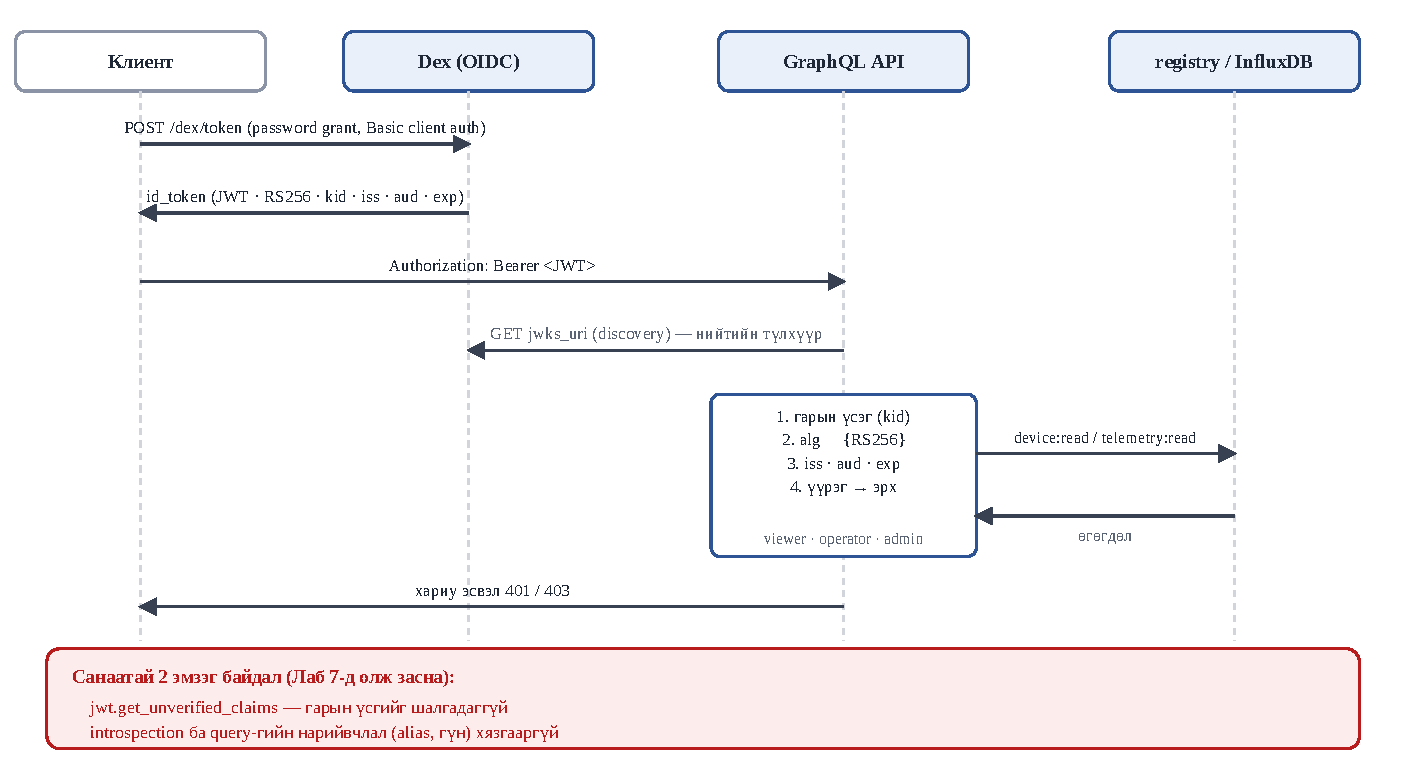
\includegraphics{figures/fig-oidc-rbac.pdf}
\caption{Зураг 7.1 --- OIDC нэвтрэлт ба RBAC: клиент → Dex (токен) → GraphQL API (JWKS-ээр гарын үсэг шалгах → үүргийн шалгалт) → бүртгэл / InfluxDB}
\end{figure}

\textbf{ID токен юугаар хамгаалагдсан бэ.} JWT нь JWS-ээр гарын үсэглэгдсэн JSON (\href{https://www.rfc-editor.org/rfc/rfc7519}{RFC 7519}, \href{https://www.rfc-editor.org/rfc/rfc7515}{RFC 7515}). OpenID Connect Core §3.1.3.7-гоор хүлээн авагч: \texttt{iss} нь issuer-тэй \textbf{яг} таарах, \texttt{aud}-д өөрийн \texttt{client\_id} байх, гарын үсгийг \textbf{issuer-ийн түлхүүрээр} (\texttt{jwks\_uri}-ээс) шалгах, одоогийн цаг \texttt{exp}-ээс өмнө байх ёстой. Толгойн \texttt{kid} нь аль түлхүүрээр гарын үсэглэснийг заах \emph{hint} л (\href{https://www.rfc-editor.org/rfc/rfc7515\#section-4.1.4}{RFC 7515 §4.1.4}); \texttt{alg}-ийг токеноос биш, \textbf{урьдчилан зөвшөөрсөн жагсаалтаас} авна (\href{https://www.rfc-editor.org/rfc/rfc8725\#section-3.1}{RFC 8725 §3.1}).

\textbf{Zero Trust:} "дотоод сүлжээ тул аюулгүй" гэсэн таамаг \textbf{байхгүй}. Хүсэлт бүрийг шалгана --- эх сурвалж хаанаас ирсэн нь хамаагүй. InfluxDB-г \texttt{-\/-without-auth} горимд ажиллуулж байгаа нь тэр зарчмыг илт зөрчсөн жишээ (Алхам 8).

\hypertarget{ux430ux43bux445ux43cux443ux443ux434}{%
\section{4. Алхмууд}\label{ux430ux43bux445ux43cux443ux443ux434}}

\hypertarget{ux430ux43bux445ux430ux43c-1-ux431ux44dux43bux442ux433ux44dux43b-ux431ux430-ux441ux445ux435ux43cux438ux439ux433-ux441ux443ux434ux43bux430ux445-15-ux43cux438ux43d-ux437ux43a}{%
\subsection{Алхам 1 --- Бэлтгэл ба схемийг судлах (15 мин) {[}ЗК{]}}\label{ux430ux43bux445ux430ux43c-1-ux431ux44dux43bux442ux433ux44dux43b-ux431ux430-ux441ux445ux435ux43cux438ux439ux433-ux441ux443ux434ux43bux430ux445-15-ux43cux438ux43d-ux437ux43a}}

Хөтчөөр \texttt{http:\allowbreak{}/\allowbreak{}/\allowbreak{}localhost:\allowbreak{}8000/\allowbreak{}graphql} нээж GraphiQL-ийг үзнэ. Токенгүйгээр зөвхөн \texttt{\{\ whoami\ \}} ажиллана. \texttt{\{\ devices(limit:\allowbreak{}\ 5)\ \{\ id\ name\ \}\ \}} бичвэл \textbf{алдаа} гарна: \texttt{\textquotesingle{}device:read\textquotesingle{}\ эрх\ байхгүй.\ Таны\ үүрэг:\ {[}{]}}. Энэ бол зөв зан төлөв --- Zero Trust-ын анхдагч: \textbf{токенгүй хүсэлт нэг ч үүрэггүй}. Тиймээс эхлээд токен авах хэрэгтэй → Алхам 2.

Схемийг GraphiQL-ийн Docs самбараас судал: \texttt{devices}, \texttt{device}, \texttt{firmware}, \texttt{anomalies}, \texttt{deviceStats} (хараахан байхгүй), \texttt{sendCommand}.

\hypertarget{ux430ux43bux445ux430ux43c-2-oidc-ux442ux43eux43aux435ux43d-ux431ux430-ux4afux4afux440ux433ux438ux439ux43d-ux44dux445-ux441ux443ux440ux432ux430ux43bux436-35-ux43cux438ux43d-ux437ux43a}{%
\subsection{Алхам 2 --- OIDC токен ба үүргийн эх сурвалж (35 мин) {[}ЗК{]}}\label{ux430ux43bux445ux430ux43c-2-oidc-ux442ux43eux43aux435ux43d-ux431ux430-ux4afux4afux440ux433ux438ux439ux43d-ux44dux445-ux441ux443ux440ux432ux430ux43bux436-35-ux43cux438ux43d-ux437ux43a}}

\textbf{2.1 Токен авах.} Dex-д гурван статик хэрэглэгч бий: \texttt{viewer@}, \texttt{operator@}, \texttt{admin@cnc302.mn}, бүгд нууц үг \texttt{cnc302}. Токены endpoint нь \texttt{\textless{}issuer\textgreater{}/\allowbreak{}token}, клиент нь \texttt{cnc302} / \texttt{cnc302-lab-secret} (\texttt{stack/\allowbreak{}dex/\allowbreak{}config.\allowbreak{}yaml}). Dex-ийн баримтын жишээний адил клиентийн нууцыг HTTP Basic-ээр (\texttt{-u}) илгээнэ:

\begin{Shaded}
\begin{Highlighting}[]
\ExtensionTok{curl} \AttributeTok{{-}s}\NormalTok{ localhost:5556/dex/.well{-}known/openid{-}configuration }\KeywordTok{|} \ExtensionTok{jq} \StringTok{\textquotesingle{}\{issuer, token\_endpoint, jwks\_uri\}\textquotesingle{}}
\FunctionTok{tok()} \KeywordTok{\{} \ExtensionTok{curl} \AttributeTok{{-}s} \AttributeTok{{-}u}\NormalTok{ cnc302:cnc302{-}lab{-}secret http://localhost:5556/dex/token }\DataTypeTok{\textbackslash{}}
  \AttributeTok{{-}{-}data{-}urlencode}\NormalTok{ grant\_type=password }\AttributeTok{{-}{-}data{-}urlencode}\NormalTok{ scope=}\StringTok{\textquotesingle{}openid email profile groups\textquotesingle{}} \DataTypeTok{\textbackslash{}}
  \AttributeTok{{-}{-}data{-}urlencode}\NormalTok{ username=}\StringTok{"}\VariableTok{$1}\StringTok{@cnc302.mn"} \AttributeTok{{-}{-}data{-}urlencode}\NormalTok{ password=cnc302 }\DataTypeTok{\textbackslash{}}
  \KeywordTok{|} \ExtensionTok{jq} \AttributeTok{{-}r}\NormalTok{ .id\_token}\KeywordTok{;} \KeywordTok{\}}
\VariableTok{TOKEN}\OperatorTok{=}\VariableTok{$(}\ExtensionTok{tok}\NormalTok{ admin}\VariableTok{)} \KeywordTok{\&\&} \BuiltInTok{echo} \StringTok{"}\VariableTok{$\{TOKEN}\OperatorTok{:}\DecValTok{0}\OperatorTok{:}\DecValTok{40}\VariableTok{\}}\StringTok{…"}
\end{Highlighting}
\end{Shaded}

\begin{quote}
Албан ёсны баримт: \href{https://dexidp.io/docs/connectors/local/}{Dex --- Local connector, Obtaining a token} · \href{https://dexidp.io/docs/configuration/oauth2/}{Dex --- OAuth2 grants}. Password grant ажиллахын тулд \texttt{enablePasswordDB:\allowbreak{}\ true} ба \texttt{oauth2.\allowbreak{}passwordConnector:\allowbreak{}\ local} хоёулаа хэрэгтэй. Dex-ийн баримтад энэ grant-ыг \emph{"not recommended"} гэж тэмдэглэсэн (OAuth 2.0 Security BCP) --- лабораторид л ашиглана; яагаад гэдгийг тайланд бич.
\end{quote}

\begin{quote}
\texttt{null} буцаавал \texttt{curl}-аас \texttt{\textbar{}\ jq\ -r\ .id\_token}-ийг хасаж алдааг хар: \texttt{invalid\_grant}/\allowbreak\texttt{Invalid\ username\ or\ password} бол \texttt{config.yaml}-ийн bcrypt hash нууц үгтэй таарахгүй; \texttt{unsupported\_\allowbreak{}grant\_\allowbreak{}type} бол \texttt{oauth2.\allowbreak{}grantTypes}-д \texttt{password} нэм.
\end{quote}

\textbf{2.2 Токеныг API-д ашиглах. 2.3 Гурван хэрэглэгчээр давтах:}

\begin{Shaded}
\begin{Highlighting}[]
\ControlFlowTok{for}\NormalTok{ U }\KeywordTok{in}\NormalTok{ viewer operator admin}\KeywordTok{;} \ControlFlowTok{do}
  \BuiltInTok{printf} \StringTok{\textquotesingle{}\%{-}9s \textquotesingle{}} \StringTok{"}\VariableTok{$U}\StringTok{"}
  \ExtensionTok{curl} \AttributeTok{{-}s} \AttributeTok{{-}X}\NormalTok{ POST localhost:8000/graphql }\AttributeTok{{-}H} \StringTok{"Authorization: Bearer }\VariableTok{$(}\ExtensionTok{tok} \VariableTok{$U)}\StringTok{"} \DataTypeTok{\textbackslash{}}
    \AttributeTok{{-}H} \StringTok{\textquotesingle{}Content{-}Type: application/json\textquotesingle{}} \AttributeTok{{-}d} \StringTok{\textquotesingle{}\{"query":"\{ whoami \}"\}\textquotesingle{}} \KeywordTok{|} \ExtensionTok{jq} \AttributeTok{{-}r}\NormalTok{ .data.whoami}
\ControlFlowTok{done}
\end{Highlighting}
\end{Shaded}

\hypertarget{ux445ux4afux441ux43dux44dux433ux442-7.1-ux442ux43eux43aux435ux43dux43eux43eux441-ux4afux4afux440ux44dux433-ux445ux4afux440ux442ux44dux43b}{%
\subsubsection{Хүснэгт 7.1 --- Токеноос үүрэг хүртэл}\label{ux445ux4afux441ux43dux44dux433ux442-7.1-ux442ux43eux43aux435ux43dux43eux43eux441-ux4afux4afux440ux44dux433-ux445ux4afux440ux442ux44dux43b}}

\begingroup\scriptsize\begin{longtable}[]{@{}
  >{\raggedright\arraybackslash}p{(\columnwidth - 6\tabcolsep) * \real{0.2500}}
  >{\raggedright\arraybackslash}p{(\columnwidth - 6\tabcolsep) * \real{0.2500}}
  >{\raggedright\arraybackslash}p{(\columnwidth - 6\tabcolsep) * \real{0.2500}}
  >{\raggedright\arraybackslash}p{(\columnwidth - 6\tabcolsep) * \real{0.2500}}@{}}
\toprule
\begin{minipage}[b]{\linewidth}\raggedright
Хэрэглэгч
\end{minipage} & \begin{minipage}[b]{\linewidth}\raggedright
\texttt{id\_token}-ы \texttt{groups} талбар байна уу
\end{minipage} & \begin{minipage}[b]{\linewidth}\raggedright
\texttt{whoami}-гийн \texttt{roles=}
\end{minipage} & \begin{minipage}[b]{\linewidth}\raggedright
\texttt{perms=} тоо
\end{minipage} \\
\midrule
\endhead
\bottomrule
\endlastfoot
viewer@cnc302.mn & & & \\
operator@cnc302.mn & & & \\
admin@cnc302.mn & & & \\
\end{longtable}\endgroup

Токеныг задлан үзэх: \texttt{echo\ "\$TOKEN"\ \textbar{}\ cut\ -d.\ -f2\ \textbar{}\ base64\ -d\ 2\textgreater{}/dev/null\ \textbar{}\ jq} (base64url тул padding дутуу бол \texttt{jq} алдаа өгч болно). Толгой: \texttt{echo\ "\$TOKEN"\ \textbar{}\ cut\ -d.\ -f1\ \textbar{}\ base64\ -d\ 2\textgreater{}/dev/null} --- \texttt{alg} ба \texttt{kid}-ийг тэмдэглэ.

\textbf{Ажиглалт:} Dex-ийн статик хэрэглэгчид (\texttt{staticPasswords}: \texttt{email}, \texttt{hash}, \texttt{username}, \texttt{userID} --- \href{https://dexidp.io/docs/connectors/local/}{Dex local connector}) бүлгийн мэдээлэлгүй тул \texttt{groups} scope хүссэн ч токенд \texttt{groups} \textbf{ирэхгүй}. \texttt{decode\_token} нь \texttt{groups} олдохгүй бол \texttt{{[}"viewer"{]}}-д унана --- тиймээс \textbf{гурвуулаа viewer} болно. \textbf{2.4:} хоёр шийдлийг харьцуулж, нэгийг нь хэрэгжүүл.

\hypertarget{ux445ux4afux441ux43dux44dux433ux442-7.2-ux4afux4afux440ux433ux438ux439ux43d-ux44dux445-ux441ux443ux440ux432ux430ux43bux436ux438ux439ux43d-ux441ux43eux43dux433ux43eux43bux442}{%
\subsubsection{Хүснэгт 7.2 --- Үүргийн эх сурвалжийн сонголт}\label{ux445ux4afux441ux43dux44dux433ux442-7.2-ux4afux4afux440ux433ux438ux439ux43d-ux44dux445-ux441ux443ux440ux432ux430ux43bux436ux438ux439ux43d-ux441ux43eux43dux433ux43eux43bux442}}

\begingroup\scriptsize\begin{longtable}[]{@{}
  >{\raggedright\arraybackslash}p{(\columnwidth - 4\tabcolsep) * \real{0.3333}}
  >{\raggedright\arraybackslash}p{(\columnwidth - 4\tabcolsep) * \real{0.3333}}
  >{\raggedright\arraybackslash}p{(\columnwidth - 4\tabcolsep) * \real{0.3333}}@{}}
\toprule
\begin{minipage}[b]{\linewidth}\raggedright
\end{minipage} & \begin{minipage}[b]{\linewidth}\raggedright
(а) Dex-д LDAP/GitHub холбогч
\end{minipage} & \begin{minipage}[b]{\linewidth}\raggedright
(б) API дээр имэйлээс үүрэг зурвасжуулах
\end{minipage} \\
\midrule
\endhead
\bottomrule
\endlastfoot
Хэрэгжүүлэх хугацаа (мин) & & \\
Үүргийг хаана удирдах вэ & & \\
Токен хуурамч бол ажиллах уу & & \\
Үйлдвэрлэлд тохирох уу & & \\
\textbf{Бидний сонголт ба шалтгаан} & & \\
\end{longtable}\endgroup

Лабораторийн цагт (б)-г хэрэгжүүлэх нь бодитой: \texttt{decode\_token}-д \texttt{claims.\allowbreak{}get("email")}-ээс \texttt{admin@} → \texttt{admin}, \texttt{operator@} → \texttt{operator} зурвасжуулна. Гэхдээ тайландаа \textbf{(а) яагаад илүү зөв болохыг} заавал бич.

\hypertarget{ux430ux43bux445ux430ux43c-3-rest-ux431ux430-graphql-ux438ux439ux43d-ux445ux430ux440ux44cux446ux443ux443ux43bux430ux43bux442-45-ux43cux438ux43d-ux437ux43a}{%
\subsection{Алхам 3 --- REST ба GraphQL-ийн харьцуулалт (45 мин) {[}ЗК{]}}\label{ux430ux43bux445ux430ux43c-3-rest-ux431ux430-graphql-ux438ux439ux43d-ux445ux430ux440ux44cux446ux443ux443ux43bux430ux43bux442-45-ux43cux438ux43d-ux437ux43a}}

\textbf{3.1 GraphQL --- нэг хүсэлт:}

\begin{Shaded}
\begin{Highlighting}[]
\BuiltInTok{time}\NormalTok{ curl }\AttributeTok{{-}s} \AttributeTok{{-}X}\NormalTok{ POST localhost:8000/graphql }\AttributeTok{{-}H} \StringTok{"Authorization: Bearer }\VariableTok{$TOKEN}\StringTok{"} \DataTypeTok{\textbackslash{}}
  \AttributeTok{{-}H} \StringTok{\textquotesingle{}Content{-}Type: application/json\textquotesingle{}} \AttributeTok{{-}o}\NormalTok{ /tmp/gql5.json }\DataTypeTok{\textbackslash{}}
  \AttributeTok{{-}d} \StringTok{\textquotesingle{}\{"query":"\{ devices(limit:5)\{ name state readings(limit:10)\{ time temperature vibrationRms \} \} \}"\}\textquotesingle{}}
\FunctionTok{wc} \AttributeTok{{-}c}\NormalTok{ /tmp/gql5.json}
\end{Highlighting}
\end{Shaded}

\textbf{3.2 REST --- 1 + N хүсэлт.} Эхлээд жагсаалт (\texttt{/rest/devices} нь ЗӨВХӨН жагсаалт буцаана), дараа нь төхөөрөмж тус бүрийн хэмжилт:

\begin{Shaded}
\begin{Highlighting}[]
\ExtensionTok{curl} \AttributeTok{{-}s} \AttributeTok{{-}H} \StringTok{"Authorization: Bearer }\VariableTok{$TOKEN}\StringTok{"} \DataTypeTok{\textbackslash{}}
  \StringTok{\textquotesingle{}localhost:8000/rest/devices?limit=5\textquotesingle{}} \KeywordTok{|} \ExtensionTok{jq} \AttributeTok{{-}r} \StringTok{\textquotesingle{}.devices[].name\textquotesingle{}} \OperatorTok{\textgreater{}}\NormalTok{ /tmp/devs.txt}
\BuiltInTok{time} \ErrorTok{(}\ControlFlowTok{while} \BuiltInTok{read} \VariableTok{d}\KeywordTok{;} \ControlFlowTok{do}
  \ExtensionTok{curl} \AttributeTok{{-}s} \AttributeTok{{-}X}\NormalTok{ POST localhost:8181/api/v3/query\_sql }\AttributeTok{{-}H} \StringTok{\textquotesingle{}Content{-}Type: application/json\textquotesingle{}} \DataTypeTok{\textbackslash{}}
    \AttributeTok{{-}d} \StringTok{"\{}\DataTypeTok{\textbackslash{}"}\StringTok{db}\DataTypeTok{\textbackslash{}"}\StringTok{:}\DataTypeTok{\textbackslash{}"}\StringTok{cnc302}\DataTypeTok{\textbackslash{}"}\StringTok{,}\DataTypeTok{\textbackslash{}"}\StringTok{q}\DataTypeTok{\textbackslash{}"}\StringTok{:}\DataTypeTok{\textbackslash{}"}\StringTok{SELECT time, temperature, vibration\_rms FROM telemetry WHERE device=\textquotesingle{}}\VariableTok{$d}\StringTok{\textquotesingle{} ORDER BY time DESC LIMIT 10}\DataTypeTok{\textbackslash{}"}\StringTok{,}\DataTypeTok{\textbackslash{}"}\StringTok{format}\DataTypeTok{\textbackslash{}"}\StringTok{:}\DataTypeTok{\textbackslash{}"}\StringTok{json}\DataTypeTok{\textbackslash{}"}\StringTok{\}"}
\ControlFlowTok{done} \OperatorTok{\textless{}}\NormalTok{ /tmp/devs.txt}\KeywordTok{)} \OperatorTok{\textgreater{}}\NormalTok{ /tmp/rest5.json}
\FunctionTok{wc} \AttributeTok{{-}l}\NormalTok{ /tmp/devs.txt }\KeywordTok{\&\&} \FunctionTok{wc} \AttributeTok{{-}c}\NormalTok{ /tmp/rest5.json}
\end{Highlighting}
\end{Shaded}

\textbf{3.3 50 төхөөрөмж дээр давт} (\texttt{limit:5} → \texttt{limit:50}). Ялгаа шугаман өсөв үү?

\hypertarget{ux445ux4afux441ux43dux44dux433ux442-7.3-rest-ux431ux430-graphql}{%
\subsubsection{Хүснэгт 7.3 --- REST ба GraphQL}\label{ux445ux4afux441ux43dux44dux433ux442-7.3-rest-ux431ux430-graphql}}

\begingroup\scriptsize\begin{longtable}[]{@{}lll@{}}
\toprule
Хэмжилт & REST & GraphQL \\
\midrule
\endhead
\bottomrule
\endlastfoot
5 төхөөрөмж: хүсэлтийн тоо & & 1 \\
5 төхөөрөмж: нийт хугацаа (мс) & & \\
50 төхөөрөмж: хүсэлтийн тоо & & 1 \\
50 төхөөрөмж: нийт хугацаа (мс) & & \\
50 төхөөрөмж: хариуны байт & & \\
Илүүдэл өгөгдөл (over-fetching) байна уу & & \\
\end{longtable}\endgroup

\begin{quote}
\textbf{Санамж:} REST-ийн хугацаа нь \texttt{localhost} дээр хамгийн таатай нөхцөлд хэмжигдэж байна. Сүлжээний саатал (RTT) 200 мс байсан бол 51 хүсэлт \textbf{дор хаяж 10 секунд} болно. Хяналтын асуулт 1-д үүнийг тоогоор гарга.
\end{quote}

\hypertarget{ux430ux43bux445ux430ux43c-4-devicestats-ux431ux430-ux43dux44dux433ux442ux433ux44dux43bux438ux439ux43d-ux431ux430ux439ux440ux43bux430ux43b-30-ux43cux438ux43d-ux437ux43a}{%
\subsection{\texorpdfstring{Алхам 4 --- \texttt{deviceStats} ба нэгтгэлийн байрлал (30 мин) {[}ЗК{]}}{Алхам 4 --- deviceStats ба нэгтгэлийн байрлал (30 мин) {[}ЗК{]}}}\label{ux430ux43bux445ux430ux43c-4-devicestats-ux431ux430-ux43dux44dux433ux442ux433ux44dux43bux438ux439ux43d-ux431ux430ux439ux440ux43bux430ux43b-30-ux43cux438ux43d-ux437ux43a}}

\texttt{main.py} дотор \texttt{\#\ TODO(оюутан)} гэсэн тэмдэглэгээ бий. Дараах талбарыг нэмнэ:

\begin{Shaded}
\begin{Highlighting}[]
\NormalTok{\{ deviceStats(device: }\StringTok{"dev0001"}\NormalTok{, hours: }\DecValTok{24}\NormalTok{) \{ avg min max samples \} \}}
\end{Highlighting}
\end{Shaded}

\textbf{Дүрэм:} нэгтгэлийг \textbf{InfluxDB-д хийлгэнэ} (SQL-ийн \texttt{avg/\allowbreak{}min/\allowbreak{}max/\allowbreak{}count}), Python дээр биш:

\begin{Shaded}
\begin{Highlighting}[]
\KeywordTok{SELECT} \FunctionTok{avg}\NormalTok{(temperature) }\KeywordTok{AS} \FunctionTok{avg}\NormalTok{, }\FunctionTok{min}\NormalTok{(temperature) }\KeywordTok{AS} \FunctionTok{min}\NormalTok{, }\FunctionTok{max}\NormalTok{(temperature) }\KeywordTok{AS} \FunctionTok{max}\NormalTok{,}
       \FunctionTok{count}\NormalTok{(temperature) }\KeywordTok{AS}\NormalTok{ samples}
\KeywordTok{FROM}\NormalTok{ telemetry }\KeywordTok{WHERE}\NormalTok{ device }\OperatorTok{=} \StringTok{\textquotesingle{}\textless{}...\textgreater{}\textquotesingle{}} \KeywordTok{AND} \DataTypeTok{time} \OperatorTok{\textgreater{}}\NormalTok{ now() }\OperatorTok{{-}} \DataTypeTok{INTERVAL} \StringTok{\textquotesingle{}24 hours\textquotesingle{}}
\end{Highlighting}
\end{Shaded}

Дараа нь дахин барина: \texttt{docker\ compose\ -\/\allowbreak{}-profile\ app\ up\ -d\ -\/\allowbreak{}-build\ graphql-api}

\textbf{Хоёр хувилбарыг хэмж:} (а) SQL-д нэгтгэх, (б) бүх мөрийг татаад Python дээр нэгтгэх.

\hypertarget{ux445ux4afux441ux43dux44dux433ux442-7.4-ux43dux44dux433ux442ux433ux44dux43bux438ux439ux433-ux445ux430ux430ux43dux430-ux445ux438ux439ux445-ux432ux44d}{%
\subsubsection{Хүснэгт 7.4 --- Нэгтгэлийг хаана хийх вэ}\label{ux445ux4afux441ux43dux44dux433ux442-7.4-ux43dux44dux433ux442ux433ux44dux43bux438ux439ux433-ux445ux430ux430ux43dux430-ux445ux438ux439ux445-ux432ux44d}}

\begingroup\scriptsize\begin{longtable}[]{@{}lll@{}}
\toprule
& InfluxDB дээр (SQL) & Python дээр (API) \\
\midrule
\endhead
\bottomrule
\endlastfoot
Хариу ирэх хугацаа (мс), 24 цаг & & \\
InfluxDB-ээс татсан мөрийн тоо & & \\
Хариуны байт & & \\
30 хоногийн өгөгдөл дээр (мс) & & \\
\end{longtable}\endgroup

\textbf{Дүгнэлт:} нэгтгэлийг өгөгдөлд ойр хийх зарчим яагаад чухал вэ: ule{1.5cm}{0.4pt}

\hypertarget{ux430ux43bux445ux430ux43c-5-ux431ux43eux434ux438ux442-ux445ux443ux433ux430ux446ux430ux430ux43dux44b-ux448ux438ux43dux44dux447ux43bux44dux43b-polling-ux431ux430-websocket-25-ux43cux438ux43d-ux437ux43a}{%
\subsection{Алхам 5 --- Бодит хугацааны шинэчлэл: polling ба WebSocket (25 мин) {[}ЗК{]}}\label{ux430ux43bux445ux430ux43c-5-ux431ux43eux434ux438ux442-ux445ux443ux433ux430ux446ux430ux430ux43dux44b-ux448ux438ux43dux44dux447ux43bux44dux43b-polling-ux431ux430-websocket-25-ux43cux438ux43d-ux437ux43a}}

\textbf{5.1 Одоогийн байдал --- polling.} 1 секунд тутам асуух:

\begin{Shaded}
\begin{Highlighting}[]
\FunctionTok{timeout}\NormalTok{ 60 bash }\AttributeTok{{-}c} \StringTok{\textquotesingle{}while true; do}
\StringTok{  curl {-}s {-}o /dev/null {-}w "\%\{size\_download\} " {-}X POST localhost:8000/graphql \textbackslash{}}
\StringTok{    {-}H "Authorization: Bearer \textquotesingle{}"}\VariableTok{$TOKEN}\StringTok{"\textquotesingle{}" {-}H "Content{-}Type: application/json" \textbackslash{}}
\StringTok{    {-}d "\{\textbackslash{}"query\textbackslash{}":\textbackslash{}"\{ devices(limit:5)\{ name \} \}\textbackslash{}"\}"; sleep 1}
\StringTok{done\textquotesingle{}} \KeywordTok{|} \FunctionTok{tr} \StringTok{\textquotesingle{} \textquotesingle{}} \StringTok{\textquotesingle{}\textbackslash{}n\textquotesingle{}} \KeywordTok{|} \FunctionTok{awk} \StringTok{\textquotesingle{}\{s+=$1; n++\} END \{print n " хүсэлт, " s " байт"\}\textquotesingle{}}
\end{Highlighting}
\end{Shaded}

\textbf{5.2 ОЮУТНЫ ДААЛГАВАР --- WebSocket.} \texttt{main.py} дотор одоо WebSocket \textbf{байхгүй}. Хоёр замын аль нэгийг сонгож нэмнэ:

\begin{itemize}
\tightlist
\item
  (а) Strawberry-гийн \texttt{@strawberry.\allowbreak{}subscription} (async generator буцаадаг resolver) + \texttt{strawberry.\allowbreak{}Schema(.\allowbreak{}.\allowbreak{}.\allowbreak{},\ subscription=\allowbreak{}Subscription)}. \texttt{GraphQLRouter} анхдагчаар \texttt{graphql-transport-ws} ба хуучин \texttt{graphql-ws} хоёр протоколыг хоёуланг нь идэвхжүүлсэн байдаг (\href{https://strawberry.rocks/docs/general/subscriptions}{Strawberry --- Subscriptions}, \href{https://strawberry.rocks/docs/integrations/fastapi}{FastAPI integration}).
\item
  (б) FastAPI-гийн \texttt{@app.\allowbreak{}websocket("/\allowbreak{}ws/\allowbreak{}telemetry")} --- \texttt{await\ websocket.\allowbreak{}accept()}, дараа нь \texttt{await\ websocket.\allowbreak{}send\_\allowbreak{}text(.\allowbreak{}.\allowbreak{}.\allowbreak{})}; клиент салахад \texttt{WebSocketDisconnect} шидэгдэнэ (\href{https://fastapi.tiangolo.com/advanced/websockets/}{FastAPI --- WebSockets}). EMQX-д paho-mqtt-ээр захиалж, ирсэн мессежийг клиент рүү түлхэнэ. paho-гийн callback тусдаа thread-д ажилладаг тул мессежийг \texttt{asyncio.Queue}-д \texttt{loop.\allowbreak{}call\_\allowbreak{}soon\_\allowbreak{}threadsafe(queue.\allowbreak{}put\_\allowbreak{}nowait,\ msg)}-ээр дамжуул.
\end{itemize}

\begin{quote}
WebSocket endpoint-д ч \texttt{Depends}, \texttt{Header}, \texttt{Query} ажилладаг (FastAPI баримт) --- \textbf{токен шалгахаа бүү март}: Zero Trust нь WebSocket-д ч хамаатай.
\end{quote}

(б) нь энэ архитектурт илүү шууд: {[}Pi{]} Pi-гийн агент → гүүр → EMQX → API → хөтөч. Дараа нь хэмжинэ:

\begin{Shaded}
\begin{Highlighting}[]
\ExtensionTok{python3} \AttributeTok{{-}} \OperatorTok{\textless{}\textless{}\textquotesingle{}EOF\textquotesingle{}}
\StringTok{import json, time, websocket        \# pip install websocket{-}client}
\StringTok{ws = websocket.create\_connection("ws://localhost:8000/ws/telemetry")}
\StringTok{t0, n, b = time.time(), 0, 0}
\StringTok{while time.time() {-} t0 \textless{} 60:}
\StringTok{    m = ws.recv(); n += 1; b += len(m)}
\StringTok{ws.close()}
\StringTok{print(f"\{n\} мессеж, \{b\} байт, 60 сек")}
\OperatorTok{EOF}
\end{Highlighting}
\end{Shaded}

\hypertarget{ux445ux4afux441ux43dux44dux433ux442-7.5-polling-ux431ux430-websocket-60-ux441ux435ux43aux443ux43dux434-5-ux442ux4e9ux445ux4e9ux4e9ux440ux4e9ux43cux436}{%
\subsubsection{Хүснэгт 7.5 --- Polling ба WebSocket (60 секунд, 5 төхөөрөмж)}\label{ux445ux4afux441ux43dux44dux433ux442-7.5-polling-ux431ux430-websocket-60-ux441ux435ux43aux443ux43dux434-5-ux442ux4e9ux445ux4e9ux4e9ux440ux4e9ux43cux436}}

\begingroup\scriptsize\begin{longtable}[]{@{}lll@{}}
\toprule
& 1 сек polling & WebSocket \\
\midrule
\endhead
\bottomrule
\endlastfoot
Хүсэлт / холболтын тоо & & 1 \\
Нийт байт & & \\
Шинэчлэлийн дундаж саатал (мс) & & \\
\end{longtable}\endgroup

\hypertarget{ux430ux43bux445ux430ux43c-6-ux430ux44eux443ux43bux433ux4afux439-ux431ux430ux439ux434ux43bux44bux43d-ux448ux430ux43bux433ux430ux43bux442-30-ux43cux438ux43d-ux437ux43a}{%
\subsection{Алхам 6 --- АЮУЛГҮЙ БАЙДЛЫН ШАЛГАЛТ (30 мин) {[}ЗК{]}}\label{ux430ux43bux445ux430ux43c-6-ux430ux44eux443ux43bux433ux4afux439-ux431ux430ux439ux434ux43bux44bux43d-ux448ux430ux43bux433ux430ux43bux442-30-ux43cux438ux43d-ux437ux43a}}

\texttt{security\_\allowbreak{}tests.\allowbreak{}py} нь \textbf{9 шалгалт} ажиллуулна. Анхаар: \texttt{-\/-tb} тугийг \texttt{-\/-registry} \textbf{орлосон} --- ThingsBoard энэ архитектурт байхгүй.

\begin{Shaded}
\begin{Highlighting}[]
\FunctionTok{mkdir} \AttributeTok{{-}p}\NormalTok{ lab07/out}
\ExtensionTok{python3}\NormalTok{ lab07/security\_tests.py }\AttributeTok{{-}{-}api}\NormalTok{ http://localhost:8000 }\DataTypeTok{\textbackslash{}}
    \AttributeTok{{-}{-}influx}\NormalTok{ http://localhost:8181 }\AttributeTok{{-}{-}registry}\NormalTok{ http://localhost:8090 }\DataTypeTok{\textbackslash{}}
    \AttributeTok{{-}{-}json}\NormalTok{ lab07/out/security{-}before.json}
\end{Highlighting}
\end{Shaded}

Гаралт \textbf{хоёр бүлэгт} тусгаарлагдана:

\begin{itemize}
\tightlist
\item
  \textbf{САНААТАЙ ЭМЗЭГ БАЙДАЛ} --- \texttt{main.py}-ийн \texttt{decode\_token}-д зориудаар үлдээсэн. \textbf{ЯГ 2} байх ёстой; өөр тоо гарвал шалгалт эсвэл API буруу ажиллаж байна.
\item
  \textbf{Дэд бүтцийн ноцтой олдвор} --- код биш, тохиргоо. Танилтгүй InfluxDB бол \textbf{бодит} асуудал, гэхдээ "тэр хоёрын" нэг \textbf{биш}. Энэ ялгааг тайланд заавал хадгал.
\end{itemize}

\textbf{Гараар давтаж батал} --- гарын үсгийн шалгалт:

\begin{Shaded}
\begin{Highlighting}[]
\ExtensionTok{python3} \AttributeTok{{-}} \OperatorTok{\textless{}\textless{}\textquotesingle{}EOF\textquotesingle{}}
\StringTok{import base64, json, time, httpx}
\StringTok{b = lambda d: base64.urlsafe\_b64encode(json.dumps(d).encode()).rstrip(b\textquotesingle{}=\textquotesingle{}).decode()}
\StringTok{sig = base64.urlsafe\_b64encode(b\textquotesingle{}not{-}a{-}real{-}signature\textquotesingle{}).rstrip(b\textquotesingle{}=\textquotesingle{}).decode()}
\StringTok{evil = f"\{b(\{\textquotesingle{}alg\textquotesingle{}:\textquotesingle{}RS256\textquotesingle{},\textquotesingle{}typ\textquotesingle{}:\textquotesingle{}JWT\textquotesingle{}\})\}.\{b(\{\textquotesingle{}sub\textquotesingle{}:\textquotesingle{}attacker\textquotesingle{},\textquotesingle{}groups\textquotesingle{}:[\textquotesingle{}admin\textquotesingle{}],\textquotesingle{}exp\textquotesingle{}:time.time()+3600\})\}.\{sig\}"}
\StringTok{r = httpx.post("http://localhost:8000/graphql", json=\{"query": "\{ whoami \}"\},}
\StringTok{               headers=\{"Authorization": f"Bearer \{evil\}"\})}
\StringTok{print(r.json())}
\OperatorTok{EOF}
\end{Highlighting}
\end{Shaded}

\texttt{roles=admin} гэж гарвал --- \textbf{та ямар ч нууц үггүйгээр админ боллоо}.

Хугацаа дууссан токеныг ч давт (\texttt{\textquotesingle{}exp\textquotesingle{}:\ time.time()\ -\ 7200}) --- мөн адил \texttt{admin} гарах ёстой. Гурав дахь халдлага: 200 давхар нэрлэсэн талбартай нэг асуулга. \texttt{security\_\allowbreak{}tests.\allowbreak{}py} нь эрх шаарддаггүй \texttt{a0:\allowbreak{}\ whoami\ …\ a199:\allowbreak{}\ whoami}-г илгээдэг --- ингэснээр шалгалт токен ба registry-ээс хамаарахгүй, зөвхөн GraphQL-ийн \textbf{валидацийн} хязгаарыг шалгана. Бодит DoS-ийг гараар давт: хүчинтэй \texttt{viewer} токентой \texttt{a0:\allowbreak{}\ devices(limit:\allowbreak{}50)\{\ name\ readings(limit:\allowbreak{}500)\{\ time\ \}\ \}\ …} илгээж хариу ирэх хугацааг тэмдэглэ.

\hypertarget{ux445ux4afux441ux43dux44dux433ux442-7.6-ux430ux44eux443ux43bux433ux4afux439-ux431ux430ux439ux434ux43bux44bux43d-9-ux448ux430ux43bux433ux430ux43bux442ux44bux43d-ux431ux4afux440ux442ux433ux44dux43b}{%
\subsubsection{Хүснэгт 7.6 --- Аюулгүй байдлын 9 шалгалтын бүртгэл}\label{ux445ux4afux441ux43dux44dux433ux442-7.6-ux430ux44eux443ux43bux433ux4afux439-ux431ux430ux439ux434ux43bux44bux43d-9-ux448ux430ux43bux433ux430ux43bux442ux44bux43d-ux431ux4afux440ux442ux433ux44dux43b}}

\begingroup\scriptsize\begin{longtable}[]{@{}
  >{\raggedright\arraybackslash}p{(\columnwidth - 14\tabcolsep) * \real{0.1250}}
  >{\raggedright\arraybackslash}p{(\columnwidth - 14\tabcolsep) * \real{0.1250}}
  >{\raggedright\arraybackslash}p{(\columnwidth - 14\tabcolsep) * \real{0.1250}}
  >{\raggedright\arraybackslash}p{(\columnwidth - 14\tabcolsep) * \real{0.1250}}
  >{\raggedright\arraybackslash}p{(\columnwidth - 14\tabcolsep) * \real{0.1250}}
  >{\raggedright\arraybackslash}p{(\columnwidth - 14\tabcolsep) * \real{0.1250}}
  >{\raggedright\arraybackslash}p{(\columnwidth - 14\tabcolsep) * \real{0.1250}}
  >{\raggedright\arraybackslash}p{(\columnwidth - 14\tabcolsep) * \real{0.1250}}@{}}
\toprule
\begin{minipage}[b]{\linewidth}\raggedright
\#
\end{minipage} & \begin{minipage}[b]{\linewidth}\raggedright
Шалгалт
\end{minipage} & \begin{minipage}[b]{\linewidth}\raggedright
Зэрэглэл
\end{minipage} & \begin{minipage}[b]{\linewidth}\raggedright
Санаатай уу
\end{minipage} & \begin{minipage}[b]{\linewidth}\raggedright
Өмнө
\end{minipage} & \begin{minipage}[b]{\linewidth}\raggedright
Хэрхэн гараар батлав
\end{minipage} & \begin{minipage}[b]{\linewidth}\raggedright
Засвар
\end{minipage} & \begin{minipage}[b]{\linewidth}\raggedright
Дараа
\end{minipage} \\
\midrule
\endhead
\bottomrule
\endlastfoot
1 & Анонимоор төхөөрөмж жагсаах татгалзсан & high & ✗ & & & & \\
2 & Хуурамч гарын үсэгтэй токен татгалзсан & \textbf{critical} & \textbf{✓} & & & & \\
3 & viewer тушаал илгээхийг татгалзсан & high & ✗ & & & & \\
4 & Хугацаа дууссан токен татгалзсан & \textbf{high} & \textbf{✓} & & & & \\
5 & Introspection хаагдсан & low & ✓ & & & & \\
6 & Асуулгын нийлмэл байдлын хязгаар & medium & ✓ & & & & \\
7 & Тарилгын оролдлого аюулгүй боловсруулагдсан & high & ✗ & & & & \\
8 & InfluxDB танилтгүй уншигдана & high & ✗ (дэд бүтэц) & & & & \\
9 & Бүртгэл танилтгүй уншигдана & medium & ✗ (дэд бүтэц) & & & & \\
\end{longtable}\endgroup

\hypertarget{ux430ux43bux445ux430ux43c-7-ux437ux430ux441ux430ux445-ux431ux430-ux434ux430ux445ux438ux43d-ux448ux430ux43bux433ux430ux445-45-ux43cux438ux43d-ux437ux43a}{%
\subsection{Алхам 7 --- ЗАСАХ ба дахин шалгах (45 мин) {[}ЗК{]}}\label{ux430ux43bux445ux430ux43c-7-ux437ux430ux441ux430ux445-ux431ux430-ux434ux430ux445ux438ux43d-ux448ux430ux43bux433ux430ux445-45-ux43cux438ux43d-ux437ux43a}}

\textbf{7.1 Гарын үсэг ба хугацааны шалгалт} (санаатай эмзэг байдал А). \texttt{jwt.\allowbreak{}get\_\allowbreak{}unverified\_\allowbreak{}claims(token)} мөрийг солино. python-jose-ийн \texttt{jwt.\allowbreak{}decode(token,\ key,\ algorithms=\allowbreak{}None,\ options=\allowbreak{}None,\ audience=\allowbreak{}None,\ issuer=\allowbreak{}None,\ subject=\allowbreak{}None,\ access\_\allowbreak{}token=\allowbreak{}None)} нь \texttt{key}-д JWK Set (\texttt{\{"keys":\allowbreak{}\ {[}.\allowbreak{}.\allowbreak{}.\allowbreak{}{]}\}}) хүлээн авна (\href{https://pypi.org/project/python-jose/}{python-jose}, \texttt{help(jose.\allowbreak{}jwt.\allowbreak{}decode)}):

\begin{Shaded}
\begin{Highlighting}[]
\ImportTok{import}\NormalTok{ time}
\ImportTok{from}\NormalTok{ jose }\ImportTok{import}\NormalTok{ JWTError, jwt}

\NormalTok{\_JWKS, \_JWKS\_AT }\OperatorTok{=} \VariableTok{None}\NormalTok{, }\FloatTok{0.0}

\KeywordTok{def}\NormalTok{ \_jwks(force: }\BuiltInTok{bool} \OperatorTok{=} \VariableTok{False}\NormalTok{) }\OperatorTok{{-}\textgreater{}} \BuiltInTok{dict}\NormalTok{:}
    \CommentTok{"""jwks\_uri{-}г discovery{-}гээс авна (OIDC Discovery), 5 минут кэшлэнэ."""}
    \KeywordTok{global}\NormalTok{ \_JWKS, \_JWKS\_AT}
    \ControlFlowTok{if}\NormalTok{ force }\KeywordTok{or}\NormalTok{ \_JWKS }\KeywordTok{is} \VariableTok{None} \KeywordTok{or}\NormalTok{ time.time() }\OperatorTok{{-}}\NormalTok{ \_JWKS\_AT }\OperatorTok{\textgreater{}} \DecValTok{300}\NormalTok{:}
\NormalTok{        conf }\OperatorTok{=}\NormalTok{ httpx.get(}\SpecialStringTok{f"}\SpecialCharTok{\{}\NormalTok{OIDC\_ISSUER}\SpecialCharTok{\}}\SpecialStringTok{/.well{-}known/openid{-}configuration"}\NormalTok{, timeout}\OperatorTok{=}\DecValTok{10}\NormalTok{).json()}
\NormalTok{        \_JWKS }\OperatorTok{=}\NormalTok{ httpx.get(conf[}\StringTok{"jwks\_uri"}\NormalTok{], timeout}\OperatorTok{=}\DecValTok{10}\NormalTok{).json()}
\NormalTok{        \_JWKS\_AT }\OperatorTok{=}\NormalTok{ time.time()}
    \ControlFlowTok{return}\NormalTok{ \_JWKS}

\NormalTok{\_VERIFY }\OperatorTok{=} \BuiltInTok{dict}\NormalTok{(}
\NormalTok{    algorithms}\OperatorTok{=}\NormalTok{[}\StringTok{"RS256"}\NormalTok{],              }\CommentTok{\# ← ЗААВАЛ: токены alg{-}д итгэхгүй}
\NormalTok{    audience}\OperatorTok{=}\StringTok{"cnc302"}\NormalTok{,                 }\CommentTok{\# Dex{-}ийн client\_id}
\NormalTok{    issuer}\OperatorTok{=}\NormalTok{OIDC\_ISSUER,                }\CommentTok{\# http://dex:5556/dex — яг таарах ёстой}
\NormalTok{    options}\OperatorTok{=}\NormalTok{\{}\StringTok{"require\_exp"}\NormalTok{: }\VariableTok{True}\NormalTok{, }\StringTok{"require\_iss"}\NormalTok{: }\VariableTok{True}\NormalTok{, }\StringTok{"require\_aud"}\NormalTok{: }\VariableTok{True}\NormalTok{,}
             \StringTok{"verify\_at\_hash"}\NormalTok{: }\VariableTok{False}\NormalTok{\}, }\CommentTok{\# доорх тайлбарыг үз}
\NormalTok{)}

\KeywordTok{def}\NormalTok{ decode\_token(token: }\BuiltInTok{str}\NormalTok{) }\OperatorTok{{-}\textgreater{}}\NormalTok{ Principal:}
    \ControlFlowTok{try}\NormalTok{:}
\NormalTok{        claims }\OperatorTok{=}\NormalTok{ jwt.decode(token, \_jwks(), }\OperatorTok{**}\NormalTok{\_VERIFY)}
    \ControlFlowTok{except}\NormalTok{ JWTError:}
        \CommentTok{\# Dex түлхүүрээ ээлжлэн солидог — шинэ kid байж магадгүй тул JWKS{-}ийг}
        \CommentTok{\# НЭГ удаа шинэчилж дахин оролдоно. Хоёр дахь алдаа → 401.}
\NormalTok{        claims }\OperatorTok{=}\NormalTok{ jwt.decode(token, \_jwks(force}\OperatorTok{=}\VariableTok{True}\NormalTok{), }\OperatorTok{**}\NormalTok{\_VERIFY)}
\NormalTok{    roles }\OperatorTok{=}\NormalTok{ claims.get(}\StringTok{"groups"}\NormalTok{) }\KeywordTok{or}\NormalTok{ claims.get(}\StringTok{"roles"}\NormalTok{) }\KeywordTok{or}\NormalTok{ [}\StringTok{"viewer"}\NormalTok{]}
\NormalTok{    ...}
\end{Highlighting}
\end{Shaded}

\begin{itemize}
\tightlist
\item
  \textbf{\texttt{algorithms=\allowbreak{}{[}"RS256"{]}}-ийг заавал заа.} Заахгүй бол халдагч \texttt{alg:\ none} (гарын үсэггүй) эсвэл \texttt{alg:\ HS256} (нийтийн түлхүүрийг HMAC-ийн нууц болгон ашиглах) халдлага хийж болно. RFC 8725 §3.1: номын сан \emph{"MUST enable the caller to specify a supported set of algorithms and MUST NOT use any other algorithms"}.
\item
  \textbf{\texttt{require\_\allowbreak{}exp:\allowbreak{}\ True}} --- python-jose-ийн анхдагч \texttt{require\_\allowbreak{}exp:\allowbreak{}\ False}: \texttt{exp}-гүй токен ч хүлээн авагдана. \texttt{verify\_exp} нь анхдагчаар асаалттай, гэхдээ \texttt{exp} \textbf{байгаа} үед л шалгана.
\item
  \textbf{\texttt{verify\_\allowbreak{}at\_\allowbreak{}hash:\allowbreak{}\ False}} --- Dex-ийн ID токенд \texttt{at\_hash} (access token-ы hash) байж болно (\href{https://dexidp.io/docs/configuration/tokens/}{Dex --- Tokens}-ийн жишээнд бий). python-jose \texttt{at\_hash} байхад \texttt{access\_token=} дамжуулахыг шаарддаг, эс бөгөөс \emph{"No access\_token provided to compare against at\_hash claim"} алдаа өгнө (бид python-jose 3.5.0 дээр туршсан). Манай API зөвхөн ID токеныг Bearer болгон авдаг тул харьцуулах access token байхгүй --- энэ шалгалтыг ухамсартайгаар унтраана. Үлдсэн шалгалт (гарын үсэг, \texttt{iss}, \texttt{aud}, \texttt{exp}) хэвээр.
\item
  \textbf{\texttt{kid}} --- python-jose JWKS-ийн түлхүүрүүдийг нэг нэгээр туршина; \texttt{kid} зөвхөн түлхүүр солигдсоныг илрүүлэхэд (дээрх дахин татах логик) хэрэгтэй.
\end{itemize}

\textbf{7.2 Introspection ба нийлмэл байдал} (санаатай эмзэг байдал Б). Strawberry-д бэлэн өргөтгөлүүд (\href{https://strawberry.rocks/docs/extensions/max-aliases-limiter}{Strawberry extensions}):

\begin{Shaded}
\begin{Highlighting}[]
\ImportTok{import}\NormalTok{ os}
\ImportTok{from}\NormalTok{ strawberry.extensions }\ImportTok{import}\NormalTok{ (DisableIntrospection, MaxAliasesLimiter,}
\NormalTok{                                   MaxTokensLimiter, QueryDepthLimiter)}

\NormalTok{exts }\OperatorTok{=}\NormalTok{ [QueryDepthLimiter(max\_depth}\OperatorTok{=}\DecValTok{6}\NormalTok{),        }\CommentTok{\# ГҮН}
\NormalTok{        MaxAliasesLimiter(max\_alias\_count}\OperatorTok{=}\DecValTok{15}\NormalTok{),  }\CommentTok{\# ӨРГӨН — шалгалт №6{-}ийн 200 alias}
\NormalTok{        MaxTokensLimiter(max\_token\_count}\OperatorTok{=}\DecValTok{1000}\NormalTok{)] }\CommentTok{\# баримтын нийт хэмжээ}
\ControlFlowTok{if}\NormalTok{ os.environ.get(}\StringTok{"ENV"}\NormalTok{, }\StringTok{"production"}\NormalTok{) }\OperatorTok{==} \StringTok{"production"}\NormalTok{:}
\NormalTok{    exts.append(DisableIntrospection())}
\NormalTok{schema }\OperatorTok{=}\NormalTok{ strawberry.Schema(query}\OperatorTok{=}\NormalTok{Query, mutation}\OperatorTok{=}\NormalTok{Mutation, extensions}\OperatorTok{=}\NormalTok{exts)}
\end{Highlighting}
\end{Shaded}

\begin{quote}
\texttt{QueryDepthLimiter} нь \textbf{гүнийг} л хязгаарлана --- 200 alias нэг түвшинд байгаа тул түүнийг зогсоохгүй. Шалгалт №6-г \texttt{MaxAliasesLimiter} (эсвэл \texttt{MaxTokensLimiter}) хаана. Тайландаа энэ ялгааг бич. \texttt{DisableIntrospection} идэвхтэй бол GraphiQL-ийн Docs самбар ажиллахгүй --- хөгжүүлэлтэд \texttt{ENV=dev} өг.
\end{quote}

\textbf{7.3 SQL мөр залгалт.} \texttt{Device.readings} дотор \texttt{self.name} шууд SQL-д залгагдаж байна. \texttt{self.name} нь бүртгэлээс ирдэг, харин бүртгэлийн \texttt{claim} нь дурын \texttt{device\_id} хүлээн авдаг (Лаб 2) --- тиймээс \texttt{x\textquotesingle{}\ OR\ \textquotesingle{}1\textquotesingle{}=\textquotesingle{}1} гэсэн нэртэй төхөөрөмж бүртгүүлж болно. Зөв засвар нь \textbf{параметржүүлсэн асуулга}: InfluxDB 3 \texttt{/\allowbreak{}api/\allowbreak{}v3/\allowbreak{}query\_\allowbreak{}sql} нь \texttt{params} объект хүлээн авч, \texttt{WHERE\ device\ =\allowbreak{}\ \$device} хэлбэрээр \textbf{зөвхөн WHERE-д} ашиглана (\href{https://docs.influxdata.com/influxdb3/core/query-data/sql/parameterized-queries/}{InfluxDB 3 --- Parameterized queries}):

\begin{Shaded}
\begin{Highlighting}[]
\NormalTok{json}\OperatorTok{=}\NormalTok{\{}\StringTok{"db"}\NormalTok{: INFLUX\_DB, }\StringTok{"q"}\NormalTok{: }\StringTok{"SELECT … FROM telemetry WHERE device = $device ORDER BY time DESC LIMIT 20"}\NormalTok{,}
      \StringTok{"params"}\NormalTok{: \{}\StringTok{"device"}\NormalTok{: }\VariableTok{self}\NormalTok{.name\}, }\StringTok{"format"}\NormalTok{: }\StringTok{"json"}\NormalTok{\}}
\end{Highlighting}
\end{Shaded}

\texttt{LIMIT} нь WHERE биш тул параметрээр өгөх боломжгүй --- \texttt{int()}-ээр хөрвүүлж, \texttt{min(limit,\ 500)} хэвээр үлдээ. (\texttt{Query.device} нь Python дээр шүүдэг тул тарилгын гадаргуугүй --- яагаад болохыг тайланд бич.) Шалгалт №7 нь энэ засварыг автоматаар илрүүлдэггүй (үргэлж АНХААР) --- засварыг кодоор нотол.

\textbf{7.4 Дахин барьж, дахин шалгана:}

\begin{Shaded}
\begin{Highlighting}[]
\ExtensionTok{docker}\NormalTok{ compose }\AttributeTok{{-}{-}profile}\NormalTok{ app up }\AttributeTok{{-}d} \AttributeTok{{-}{-}build}\NormalTok{ graphql{-}api}
\FunctionTok{sleep}\NormalTok{ 10}
\ExtensionTok{python3}\NormalTok{ lab07/security\_tests.py }\AttributeTok{{-}{-}api}\NormalTok{ http://localhost:8000 }\DataTypeTok{\textbackslash{}}
    \AttributeTok{{-}{-}influx}\NormalTok{ http://localhost:8181 }\AttributeTok{{-}{-}registry}\NormalTok{ http://localhost:8090 }\DataTypeTok{\textbackslash{}}
    \AttributeTok{{-}{-}json}\NormalTok{ lab07/out/security{-}after.json}
\end{Highlighting}
\end{Shaded}

\textbf{Хүлээгдэх:} \texttt{✓\ Санаатай\ эмзэг\ байдал\ илрээгүй\ —\ засвар\ ажиллаж\ байна.\allowbreak{}}, Introspection ба нийлмэл байдлын мөрүүд ТЭНЦСЭН. Бүх бодит токен татгалзвал \texttt{aud}/\allowbreak\texttt{iss} таарахгүй байна: токеныг хостоос \texttt{localhost:5556}-аар авсан ч \texttt{iss} нь config-ийн \texttt{issuer:\allowbreak{}\ http:\allowbreak{}/\allowbreak{}/\allowbreak{}dex:\allowbreak{}5556/\allowbreak{}dex} байдаг тул \texttt{OIDC\_ISSUER} яг тэр утгатай байх ёстой; \texttt{aud} нь \texttt{client\_id} (\texttt{cnc302}). API-гийн логийг \texttt{docker\ compose\ logs\ graphql-api}-аар хар.

\textbf{7.5 RBAC-ыг бодитоор турш:}

\begin{Shaded}
\begin{Highlighting}[]
\ControlFlowTok{for}\NormalTok{ U }\KeywordTok{in}\NormalTok{ viewer operator admin}\KeywordTok{;} \ControlFlowTok{do}
  \BuiltInTok{echo} \StringTok{"── }\VariableTok{$U}\StringTok{ ──"}
  \ExtensionTok{curl} \AttributeTok{{-}s} \AttributeTok{{-}X}\NormalTok{ POST localhost:8000/graphql }\AttributeTok{{-}H} \StringTok{"Authorization: Bearer }\VariableTok{$(}\ExtensionTok{tok} \VariableTok{$U)}\StringTok{"} \DataTypeTok{\textbackslash{}}
    \AttributeTok{{-}H} \StringTok{\textquotesingle{}Content{-}Type: application/json\textquotesingle{}} \DataTypeTok{\textbackslash{}}
    \AttributeTok{{-}d} \StringTok{\textquotesingle{}\{"query":"mutation \{ sendCommand(device:\textbackslash{}"dev0001\textbackslash{}", command:\textbackslash{}"reboot\textbackslash{}") \}"\}\textquotesingle{}} \KeywordTok{|} \ExtensionTok{jq} \AttributeTok{{-}c}
\ControlFlowTok{done}
\end{Highlighting}
\end{Shaded}

\hypertarget{ux445ux4afux441ux43dux44dux433ux442-7.7-rbac-ux43cux430ux442ux440ux438ux446}{%
\subsubsection{Хүснэгт 7.7 --- RBAC матриц}\label{ux445ux4afux441ux43dux44dux433ux442-7.7-rbac-ux43cux430ux442ux440ux438ux446}}

\begingroup\scriptsize\begin{longtable}[]{@{}lllll@{}}
\toprule
Үйлдэл & viewer & operator & admin & Бодитоор туршсан үр дүн \\
\midrule
\endhead
\bottomrule
\endlastfoot
\texttt{devices} жагсаах & ✓ & ✓ & ✓ & \\
\texttt{readings} унших & ✓ & ✓ & ✓ & \\
\texttt{sendCommand} & ✗ & ✓ & ✓ & \\
Төхөөрөмж үүсгэх / устгах & ✗ & ✗ & ✓ & \\
Бүртгэлд шууд хандах (:8090) & ? & ? & ? & \\
\end{longtable}\endgroup

Сүүлийн мөр нь \textbf{defence in depth}-ийн асуулт: RBAC зөвхөн GraphQL давхаргад л байгаа бол хэн ч :8090 руу шууд хандаж чадна.

\hypertarget{ux430ux43bux445ux430ux43c-8-influxdb---without-auth-ux431ux430-zero-trust-10-ux43cux438ux43d-ux437ux43a}{%
\subsection{\texorpdfstring{Алхам 8 --- InfluxDB \texttt{-\/-without-auth} ба Zero Trust (10 мин) {[}ЗК{]}}{Алхам 8 --- InfluxDB -\/-without-auth ба Zero Trust (10 мин) {[}ЗК{]}}}\label{ux430ux43bux445ux430ux43c-8-influxdb---without-auth-ux431ux430-zero-trust-10-ux43cux438ux43d-ux437ux43a}}

Энэ курс эхнээс нь InfluxDB-г танилтгүй ажиллуулж ирсэн. Яагаад, ямар үнээр:

\begin{Shaded}
\begin{Highlighting}[]
\ExtensionTok{curl} \AttributeTok{{-}s} \AttributeTok{{-}X}\NormalTok{ POST localhost:8181/api/v3/query\_sql }\AttributeTok{{-}H} \StringTok{\textquotesingle{}Content{-}Type: application/json\textquotesingle{}} \DataTypeTok{\textbackslash{}}
  \AttributeTok{{-}d} \StringTok{\textquotesingle{}\{"db":"cnc302","q":"SELECT count(*) FROM telemetry","format":"json"\}\textquotesingle{}} \KeywordTok{|} \ExtensionTok{jq}
\end{Highlighting}
\end{Shaded}

\hypertarget{ux445ux4afux441ux43dux44dux433ux442-7.8-ux437ux430ux441ux432ux430ux440ux44bux43d-ux4e9ux43cux43dux4e9ux445ux434ux430ux440ux430ux430ux445-ux434ux4afux43d}{%
\subsubsection{Хүснэгт 7.8 --- Засварын өмнөх/дараах дүн}\label{ux445ux4afux441ux43dux44dux433ux442-7.8-ux437ux430ux441ux432ux430ux440ux44bux43d-ux4e9ux43cux43dux4e9ux445ux434ux430ux440ux430ux430ux445-ux434ux4afux43d}}

\begingroup\scriptsize\begin{longtable}[]{@{}lll@{}}
\toprule
& Өмнө (\texttt{security-before.\allowbreak{}json}) & Дараа (\texttt{security-after.\allowbreak{}json}) \\
\midrule
\endhead
\bottomrule
\endlastfoot
ТЭНЦСЭН & & \\
АНХААР & & \\
УНАСАН & & \\
\texttt{deliberate\_\allowbreak{}criticals} & \textbf{2} & \textbf{0} \\
\texttt{infra\_criticals} & & \\
\end{longtable}\endgroup

\textbf{Тайландаа заавал хариул:} яагаад \texttt{-\/-without-auth} нь лабораторид зөвшөөрөгдөх, гэхдээ үйлдвэрлэлд болохгүй вэ? Zero Trust бол юуг шаардах байсан бэ --- гурав нэрлэ (жишээ: үйлчилгээ бүрт өөрийн таних тэмдэг, mTLS эсвэл токен, хамгийн бага эрхийн зарчим, хандалтын аудит лог).

\hypertarget{ux430ux43bux445ux430ux43c-9-git-commit-5-ux43cux438ux43d}{%
\subsection{Алхам 9 --- Git commit (5 мин)}\label{ux430ux43bux445ux430ux43c-9-git-commit-5-ux43cux438ux43d}}

\begin{Shaded}
\begin{Highlighting}[]
\BuiltInTok{cd}\NormalTok{ \textasciitilde{}/cnc302 }\KeywordTok{\&\&} \FunctionTok{git}\NormalTok{ add lab07/ stack/dex/}
\FunctionTok{git}\NormalTok{ commit }\AttributeTok{{-}m} \StringTok{"Лаб 7: GraphQL давхарга, OIDC, хоёр эмзэг байдал засагдсан"}
\FunctionTok{git}\NormalTok{ tag lab07{-}done }\KeywordTok{\&\&} \FunctionTok{git}\NormalTok{ push }\KeywordTok{\&\&} \FunctionTok{git}\NormalTok{ push }\AttributeTok{{-}{-}tags}

\CommentTok{\# ⚠ Нууц ороогүйг ЗААВАЛ шалга — хоёулаа хоосон байх ЁСТОЙ}
\FunctionTok{git}\NormalTok{ ls{-}files }\KeywordTok{|} \FunctionTok{grep} \AttributeTok{{-}E} \StringTok{\textquotesingle{}\textbackslash{}.env$|\textbackslash{}.key$|devices\textbackslash{}.csv\textquotesingle{}}
\FunctionTok{grep} \AttributeTok{{-}rn} \StringTok{\textquotesingle{}eyJ\textquotesingle{}}\NormalTok{ lab07/out/ }\KeywordTok{|} \FunctionTok{head}          \CommentTok{\# JWT{-}г тайланд бүү үлдээ}
\end{Highlighting}
\end{Shaded}

\hypertarget{ux445ux44fux43dux430ux43bux442ux44bux43d-ux430ux441ux443ux443ux43bux442ux443ux443ux434}{%
\section{5. Хяналтын асуултууд}\label{ux445ux44fux43dux430ux43bux442ux44bux43d-ux430ux441ux443ux443ux43bux442ux443ux443ux434}}

Хариулт бүр \textbf{хүснэгтээс тоо иш татсан} байх ёстой.

\begin{enumerate}
\def\labelenumi{\arabic{enumi}.}
\item
  Хүснэгт 7.3-д 50 төхөөрөмж дээр REST ба GraphQL-ийн хугацааны ялгаа хэдэн мс байв? Сүлжээний RTT 200 мс байсан бол REST хэдэн секунд болох вэ (51 × RTT)? GraphQL хэд вэ?
\item
  Хүснэгт 7.4-т нэгтгэлийг InfluxDB дээр хийхэд хэдэн дахин хурдан байв, татсан мөрийн тоо хэдэн дахин багассан бэ? 30 хоногийн өгөгдөл дээр энэ харьцаа хэрхэн өөрчлөгдсөн бэ?
\item
  Хүснэгт 7.5-д polling ба WebSocket-ийн байтын ялгаа хэд байв? 1000 хэрэглэгчтэй үед polling серверт хэдэн хүсэлт/секунд өгөх вэ?
\item
  Хүснэгт 7.6-д \textbf{санаатай} эмзэг байдал хэд байв, \textbf{дэд бүтцийн} олдвор хэд байв? Эдгээрийг яагаад ялгаж дүгнэх шаардлагатай вэ? (Санамж: аль нь код засаж, аль нь тохиргоо засаж шийдэгддэг вэ.)
\item
  \texttt{algorithms=\allowbreak{}{[}"RS256"{]}}-ийг заахгүй бол ямар хоёр халдлага боломжтой болох вэ? \texttt{alg:\ none} ба \texttt{alg:\ HS256} халдлагыг тус тус тайлбарла.
\item
  Токеныг цуцлах (revoke) хэрхэн ажилладаг вэ? JWT нь \textbf{төлөвгүй} тул энэ яагаад хэцүү вэ? Лаб 2-ын сертификат цуцлалт (Хүснэгт 2.7) болон MQTT session цуцлалттай ямар төстэй вэ?
\item
  Хүснэгт 7.7-гийн сүүлийн мөр: \texttt{viewer} эрхтэй хэрэглэгч :8090 эсвэл :8181 руу шууд хандаж чадвал RBAC ямар утгатай вэ? Zero Trust-д үүнийг хэрхэн хаах вэ (Хүснэгт 7.8-ын гурван шаардлагыг иш тат)?
\end{enumerate}

\hypertarget{ux445ux4afux43bux44dux44dux43bux433ux44dux43d-ux4e9ux433ux4e9ux445-ux437ux4afux439ux43b}{%
\section{6. Хүлээлгэн өгөх зүйл}\label{ux445ux4afux43bux44dux44dux43bux433ux44dux43d-ux4e9ux433ux4e9ux445-ux437ux4afux439ux43b}}

\begingroup\scriptsize\begin{longtable}[]{@{}
  >{\raggedright\arraybackslash}p{(\columnwidth - 4\tabcolsep) * \real{0.3333}}
  >{\raggedright\arraybackslash}p{(\columnwidth - 4\tabcolsep) * \real{0.3333}}
  >{\raggedright\arraybackslash}p{(\columnwidth - 4\tabcolsep) * \real{0.3333}}@{}}
\toprule
\begin{minipage}[b]{\linewidth}\raggedright
\#
\end{minipage} & \begin{minipage}[b]{\linewidth}\raggedright
Зүйл
\end{minipage} & \begin{minipage}[b]{\linewidth}\raggedright
Байрлал
\end{minipage} \\
\midrule
\endhead
\bottomrule
\endlastfoot
1 & Тайлан (Хүснэгт 7.1--7.8 бөглөсөн) & \texttt{lab07/report.md} → PDF \\
2 & Шалгалтын өмнөх/дараах JSON & \texttt{lab07/\allowbreak{}out/\allowbreak{}security-before.\allowbreak{}json}, \texttt{security-after.\allowbreak{}json} \\
3 & \texttt{decode\_token} ба схемийн засвар (diff хэлбэрээр) & тайлангийн хавсралт \\
4 & \texttt{deviceStats} ба WebSocket/subscription хэрэгжүүлэлт & \texttt{lab07/\allowbreak{}graphql-api/\allowbreak{}main.\allowbreak{}py} \\
5 & Git tag & \texttt{lab07-done} \\
\end{longtable}\endgroup

\hypertarget{ux4afux43dux44dux43bux433ux44dux44dux43dux438ux439-ux448ux430ux43bux433ux443ux443ux440-10-ux43eux43dux43eux43e}{%
\section{7. Үнэлгээний шалгуур (10 оноо)}\label{ux4afux43dux44dux43bux433ux44dux44dux43dux438ux439-ux448ux430ux43bux433ux443ux443ux440-10-ux43eux43dux43eux43e}}

\begingroup\scriptsize\begin{longtable}[]{@{}
  >{\raggedright\arraybackslash}p{(\columnwidth - 2\tabcolsep) * \real{0.5000}}
  >{\raggedright\arraybackslash}p{(\columnwidth - 2\tabcolsep) * \real{0.5000}}@{}}
\toprule
\begin{minipage}[b]{\linewidth}\raggedright
Шалгуур
\end{minipage} & \begin{minipage}[b]{\linewidth}\raggedright
Оноо
\end{minipage} \\
\midrule
\endhead
\bottomrule
\endlastfoot
REST/GraphQL харьцуулалт хэмжигдэж, \texttt{deviceStats} хэрэгжсэн & 2 \\
OIDC нэвтрэлт ажиллаж, үүргийн эх сурвалж шийдэгдсэн & 1 \\
Хоёр санаатай эмзэг байдал олдож, \textbf{гараар} батлагдсан & 2 \\
Засвар кодод хэрэгжиж, \texttt{security-after} дээр \texttt{deliberate\_\allowbreak{}criticals\ =\allowbreak{}\ 0} & 3 \\
WebSocket / subscription ажиллаж, Хүснэгт 7.5 бөглөгдсөн & 1 \\
RBAC матриц бодитоор туршсан, Zero Trust дүгнэлт үндэслэлтэй & 1 \\
\end{longtable}\endgroup

\textbf{Автомат 0 оноо:} засварыг зөвхөн тайланд бичээд кодод хэрэгжүүлээгүй бол.

\hypertarget{ux442ux4afux433ux44dux44dux43cux44dux43b-ux430ux43bux434ux430ux430}{%
\section{8. Түгээмэл алдаа}\label{ux442ux4afux433ux44dux44dux43cux44dux43b-ux430ux43bux434ux430ux430}}

\begingroup\scriptsize\begin{longtable}[]{@{}
  >{\raggedright\arraybackslash}p{(\columnwidth - 4\tabcolsep) * \real{0.3333}}
  >{\raggedright\arraybackslash}p{(\columnwidth - 4\tabcolsep) * \real{0.3333}}
  >{\raggedright\arraybackslash}p{(\columnwidth - 4\tabcolsep) * \real{0.3333}}@{}}
\toprule
\begin{minipage}[b]{\linewidth}\raggedright
Шинж
\end{minipage} & \begin{minipage}[b]{\linewidth}\raggedright
Шалтгаан
\end{minipage} & \begin{minipage}[b]{\linewidth}\raggedright
Шийдэл
\end{minipage} \\
\midrule
\endhead
\bottomrule
\endlastfoot
\texttt{graphql-api} эхлэхгүй & build алдаа & \texttt{docker\ compose\ logs\ graphql-api} \\
\texttt{\{\ devices\ \}} → эрх байхгүй & токенгүй хүсэлт & Алхам 2-оор токен ав \\
Dex \texttt{password} grant татгалзана (\texttt{unsupported\_\allowbreak{}grant\_\allowbreak{}type}) & grant идэвхгүй & \texttt{enablePasswordDB:\allowbreak{}\ true} + \texttt{oauth2.\allowbreak{}passwordConnector:\allowbreak{}\ local}; шаардлагатай бол \texttt{oauth2.\allowbreak{}grantTypes}-д \texttt{password} \\
Dex \texttt{invalid\_grant} / нууц үг буруу & \texttt{config.yaml}-ийн bcrypt hash \texttt{cnc302}-той таарахгүй & hash-ыг дахин үүсгэ (\texttt{htpasswd\ -bnBC\ 10\ ""\ cnc302\ \textbackslash{}\textbar{}\ tr\ -d\ \textquotesingle{}:\textbackslash{}n\textquotesingle{}}), \texttt{docker\ compose\ restart\ dex} \\
Засварын дараа бүх бодит токен 401: \texttt{No\ access\_\allowbreak{}token\ provided\ to\ compare\ against\ at\_\allowbreak{}hash\ claim} & python-jose \texttt{at\_hash}-ыг шалгаж байна & \texttt{options=\allowbreak{}\{"verify\_\allowbreak{}at\_\allowbreak{}hash":\allowbreak{}\ False\}} (Алхам 7.1) \\
Засварын дараа 401: \texttt{Invalid\ audience} / \texttt{Invalid\ issuer} & \texttt{audience}/\allowbreak\texttt{OIDC\_ISSUER} токентой таарахгүй & \texttt{aud} = \texttt{cnc302}, \texttt{iss} = \texttt{http:\allowbreak{}/\allowbreak{}/\allowbreak{}dex:\allowbreak{}5556/\allowbreak{}dex} \\
\texttt{whoami} үргэлж \texttt{viewer} & Dex статик хэрэглэгчид \texttt{groups} байхгүй & Алхам 2.3--2.4 \\
JWKS татагдахгүй & \texttt{OIDC\_ISSUER} буруу & контейнер дотроос \texttt{http:\allowbreak{}/\allowbreak{}/\allowbreak{}dex:\allowbreak{}5556/\allowbreak{}dex} байх ёстой \\
\texttt{readings} хоосон & {[}Pi{]} агент зогссон / гүүр тасарсан & {[}Pi{]} \texttt{make\ link} → \texttt{bridge/state\ 1} \\
Шалгалт "санаатай 0" гэнэ (засварын өмнө) & API дахин баригдаагүй & \texttt{up\ -d\ -\/\allowbreak{}-build\ graphql-api} \\
\end{longtable}\endgroup

\hypertarget{ux44dux445-ux441ux443ux440ux432ux430ux43bux436}{%
\section{9. Эх сурвалж}\label{ux44dux445-ux441ux443ux440ux432ux430ux43bux436}}

\begingroup\scriptsize\begin{longtable}[]{@{}
  >{\raggedright\arraybackslash}p{(\columnwidth - 6\tabcolsep) * \real{0.2500}}
  >{\raggedright\arraybackslash}p{(\columnwidth - 6\tabcolsep) * \real{0.2500}}
  >{\raggedright\arraybackslash}p{(\columnwidth - 6\tabcolsep) * \real{0.2500}}
  >{\raggedright\arraybackslash}p{(\columnwidth - 6\tabcolsep) * \real{0.2500}}@{}}
\toprule
\begin{minipage}[b]{\linewidth}\raggedright
\#
\end{minipage} & \begin{minipage}[b]{\linewidth}\raggedright
Эх сурвалж
\end{minipage} & \begin{minipage}[b]{\linewidth}\raggedright
Юуг баталгаажуулсан
\end{minipage} & \begin{minipage}[b]{\linewidth}\raggedright
Хандсан
\end{minipage} \\
\midrule
\endhead
\bottomrule
\endlastfoot
1 & \href{https://dexidp.io/docs/configuration/oauth2/}{Dex --- OAuth2} & \texttt{grantTypes} (анхдагч жагсаалтад \texttt{password} байхгүй), \texttt{passwordConnector} password grant-д заавал, \texttt{skipApprovalScreen}, password grant "not recommended" & 2026-09 \\
2 & \href{https://dexidp.io/docs/connectors/local/}{Dex --- Local connector} & \texttt{enablePasswordDB}, \texttt{staticPasswords} талбарууд, \texttt{\textless{}issuer\textgreater{}/\allowbreak{}token}-оор password grant авах жишээ (Basic auth) & 2026-09 \\
3 & \href{https://dexidp.io/docs/configuration/custom-scopes-claims-clients/}{Dex --- Scopes and Claims} & \texttt{openid\ email\ profile\ groups} scope, \texttt{groups} claim & 2026-09 \\
4 & \href{https://dexidp.io/docs/configuration/tokens/}{Dex --- Tokens} & ID токены бүтэц (\texttt{iss}, \texttt{aud}, \texttt{exp}, \texttt{at\_hash}), түлхүүрийн ээлжлэлт & 2026-09 \\
5 & \href{https://openid.net/specs/openid-connect-core-1_0.html}{OpenID Connect Core 1.\allowbreak{}0 §3.\allowbreak{}1.\allowbreak{}3.\allowbreak{}7} & ID токены шалгалтын дүрэм (\texttt{iss}, \texttt{aud}, гарын үсэг, \texttt{exp}) & 2026-09 \\
6 & \href{https://openid.net/specs/openid-connect-discovery-1_0.html}{OpenID Connect Discovery 1.\allowbreak{}0} & \texttt{jwks\_uri} & 2026-09 \\
7 & \href{https://www.rfc-editor.org/rfc/rfc7519}{RFC 7519 --- JWT} & \texttt{exp} claim & 2026-09 \\
8 & \href{https://www.rfc-editor.org/rfc/rfc7515}{RFC 7515 --- JWS} & \texttt{kid} толгой --- hint & 2026-09 \\
9 & \href{https://www.rfc-editor.org/rfc/rfc8725}{RFC 8725 --- JWT Best Current Practices} & алгоритмын зөвшөөрөгдсөн жагсаалт & 2026-09 \\
10 & \href{https://pypi.org/project/python-jose/}{python-jose (PyPI)} ба 3.5.0-ийн \texttt{jwt.decode} docstring & \texttt{jwt.\allowbreak{}decode(token,\ key,\ algorithms,\ options,\ audience,\ issuer,\ subject,\ access\_\allowbreak{}token)}, JWK Set, \texttt{options}-ийн анхдагч утгууд, \texttt{at\_hash} шаардлага. (python-jose.readthedocs.io-ийн API хуудас хоосон --- 0.2.0) & 2026-09 \\
11 & \href{https://strawberry.rocks/docs/extensions/query-depth-limiter}{Strawberry --- Query Depth Limiter} · \href{https://strawberry.rocks/docs/extensions/max-aliases-limiter}{Max Aliases Limiter} · \href{https://strawberry.rocks/docs/extensions/max-tokens-limiter}{Max Tokens Limiter} · \href{https://strawberry.rocks/docs/extensions/disable-introspection}{Disable Introspection} & өргөтгөлийн нэр ба параметр & 2026-09 \\
12 & \href{https://strawberry.rocks/docs/integrations/fastapi}{Strawberry --- FastAPI integration} · \href{https://strawberry.rocks/docs/general/subscriptions}{Subscriptions} · \href{https://strawberry.rocks/docs/types/resolvers}{Resolvers} & \texttt{GraphQLRouter}, \texttt{context\_getter}, \texttt{graphql-transport-ws}/\allowbreak\texttt{graphql-ws}, \texttt{strawberry.Info} & 2026-09 \\
13 & \href{https://fastapi.tiangolo.com/advanced/websockets/}{FastAPI --- WebSockets} & \texttt{@app.websocket}, \texttt{accept}/\allowbreak\texttt{send\_text}, \texttt{WebSocketDisconnect}, \texttt{Depends}/\allowbreak\texttt{Header} & 2026-09 \\
14 & \href{https://docs.influxdata.com/influxdb3/core/query-data/execute-queries/influxdb-v3-api/}{InfluxDB 3 Core --- Query with the HTTP API} & \texttt{POST\ /\allowbreak{}api/\allowbreak{}v3/\allowbreak{}query\_\allowbreak{}sql} (\texttt{db}, \texttt{q}, \texttt{format}, \texttt{params}) & 2026-09 \\
15 & \href{https://docs.influxdata.com/influxdb3/core/query-data/sql/parameterized-queries/}{InfluxDB 3 Core --- Parameterized SQL queries} & \texttt{\$name} параметр, зөвхөн WHERE-д & 2026-09 \\
16 & \href{https://docs.influxdata.com/influxdb3/core/reference/config-options/}{InfluxDB 3 Core --- Configuration options} & \texttt{-\/-without-auth}, \texttt{-\/\allowbreak{}-disable-authz} (health, ping, metrics) & 2026-09 \\
\end{longtable}\endgroup
